\documentclass{article}
\begin{document}

\section{Math Example}

Hello $x^2$

\section{TikZ Example}

Here is a circle with a line:

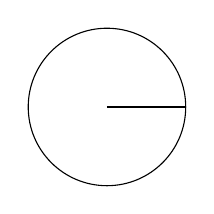
\begin{tikzpicture}
	\draw (0,0) circle (1cm);
	\draw (0,0) -- (1,0);
\end{tikzpicture}

And here is a more complex diagram:

\begin{tikzpicture}
	\def \n {5}
	\def \radius {3cm}
	\def \margin {8}

	\foreach \s in {1,...,\n}
	{
	\node[draw, circle] at ({360/\n * (\s - 1)}:\radius) {$\s$};
	\draw[->, >=latex] ({360/\n * (\s - 1)+\margin}:\radius)
	arc ({360/\n * (\s - 1)+\margin}:{360/\n * (\s)-\margin}:\radius);
	}
\end{tikzpicture}

\end{document}
